% !TEX root = ../swarthmore_talk.tex

% Elliptic Curves
\begin{frame}[plain] 
\ctext{Elliptic Curves}
\end{frame}



% EC Definition
\begin{frame}[plain]
\begin{dfn}[Elliptic Curve]
An elliptic curve is\dots
\begin{itemize}
\item A nonsingular projective curve of genus 1.
\item An abelian variety of dimension 1.
\item A nonempty smooth variety, $V(F)$, with $\deg F=3$.
\item A compact Riemann surface of genus 1.
\item The set of solutions to\dots
	\[
	y^2 + a_1 xy + a_3y = x^3 + a_2 x^2 + a_4 x + a_6
	\]
along with a specified `distinguished point $\infty$' and an addition law given by the chord-tangent law.
\end{itemize}
\end{dfn}
\end{frame}



% Cubic Functions/Elliptic Curves
\begin{frame}[plain]
\frametitle{\textcolor{white}{$n=2, d=3$: $F(x,y)=0$}---Elliptic Curves}
	\[
	y^2 + a_1 xy + a_3y = x^3 + a_2 x^2 + a_4 x + a_6
	\] \pspace 

\begin{itemize}
\item Make the substitution $y \mapsto y + \dfrac{a_1 x+a_3}{2}$.
\item Obtain $y^2= x^3+ a_2' x^2 + a_4' x + a_6'$
\item Make the substitution $x \mapsto x + \dfrac{a_2'}{3}$
\end{itemize} \pspace 
	\[
	\star \enskip \boxed{E_{A,B}: y^2 = x^3 + Ax + B} \enskip \star
	\] \pspace

\begin{itemize}
\item Require $\Delta= -16(4A^3+27B^2) \neq 0$.
\item $C(\Q)$ could be empty, finite, or infinite. 
\end{itemize}
\end{frame}



% Real Plot 
\begin{frame}[plain]
	\begin{figure}[h]
	\centering
	\begin{subfigure}{0.30\textwidth}
	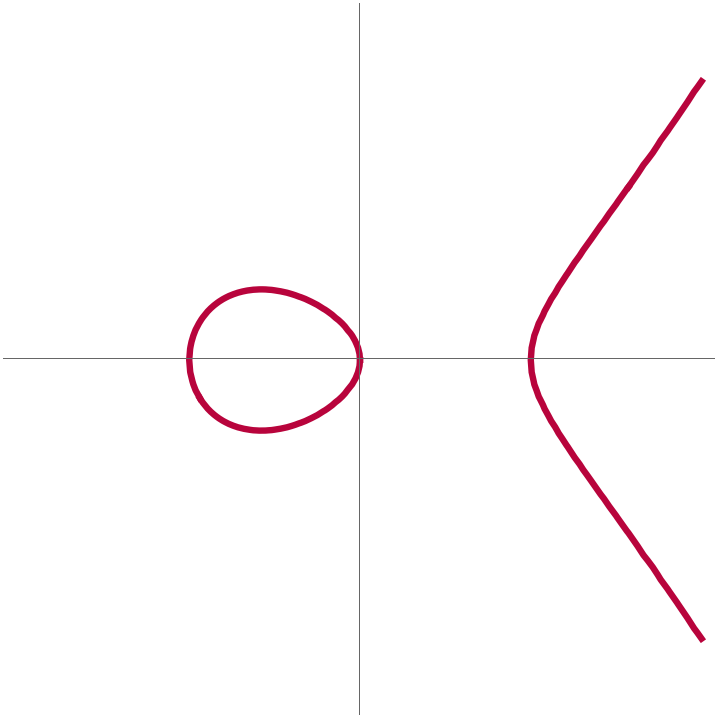
\includegraphics[width=\textwidth]{images/ec1.png}
	\caption*{$y^2 = x(x + 1)(x - 1)$}
	\end{subfigure} \qquad\qquad
	%
	\begin{subfigure}{0.30\textwidth}
	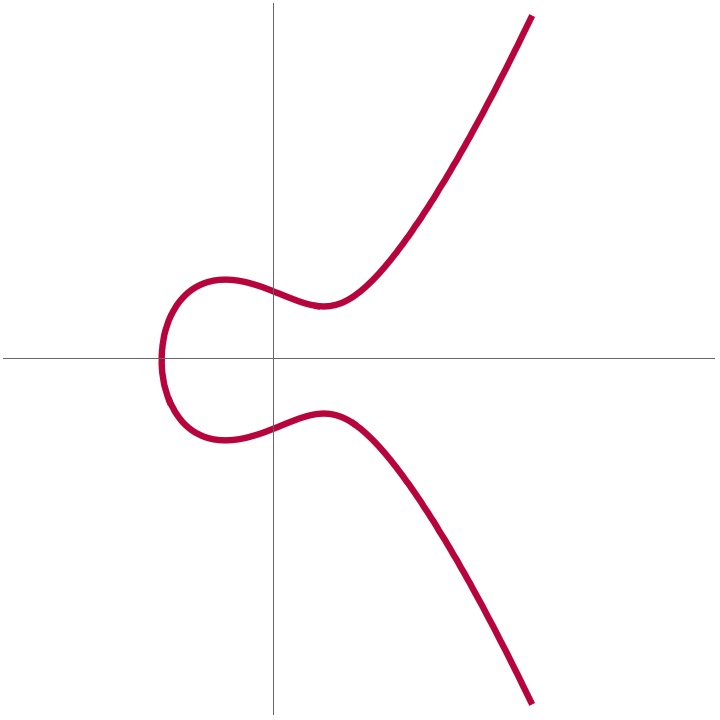
\includegraphics[width=\textwidth]{images/ec2.png}
	\caption*{$y^2 = x^3 - x + 1$}
	\end{subfigure}
	\end{figure}
	%
	\begin{figure}
	\centering
	\begin{subfigure}{0.30\textwidth}
	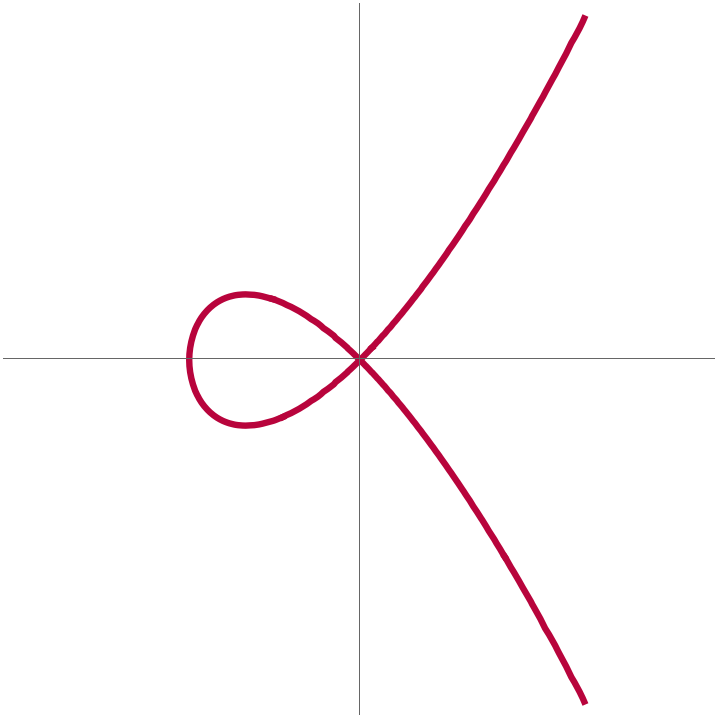
\includegraphics[width=\textwidth]{images/ec3.png}
	\caption*{$y^2 = x^2 (x + 1)$}
	\end{subfigure} \qquad\qquad
	%
	\begin{subfigure}{0.30\textwidth}
	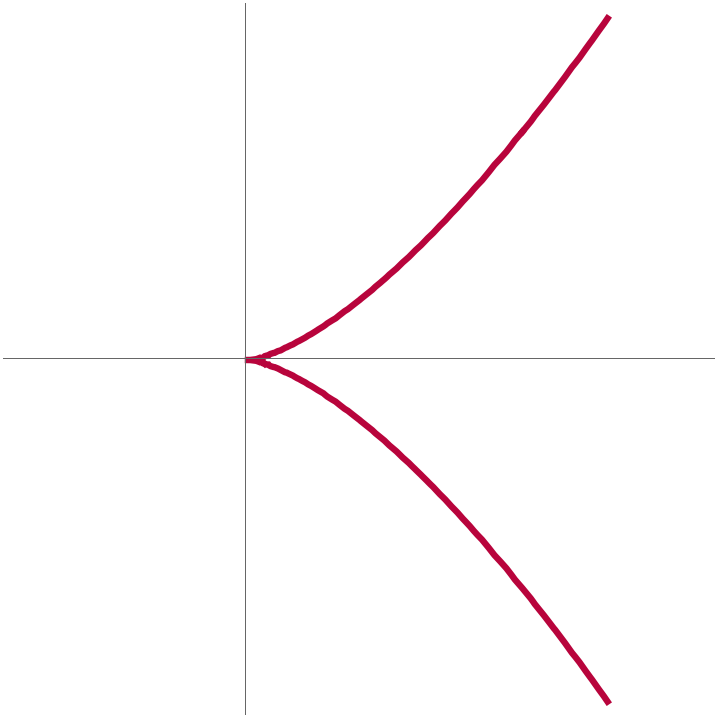
\includegraphics[width=\textwidth]{images/ec4.png}
	\caption*{$y^2= x^3$}
	\end{subfigure}
	\end{figure}
\end{frame}



% Torus
\begin{frame}[plain]
\scriptsize In fact, if one considers the complex solutions to these equations, one can show that $E(\C)$ is isomorphic to a torus!

	\begin{figure}[!ht]
	\centering
	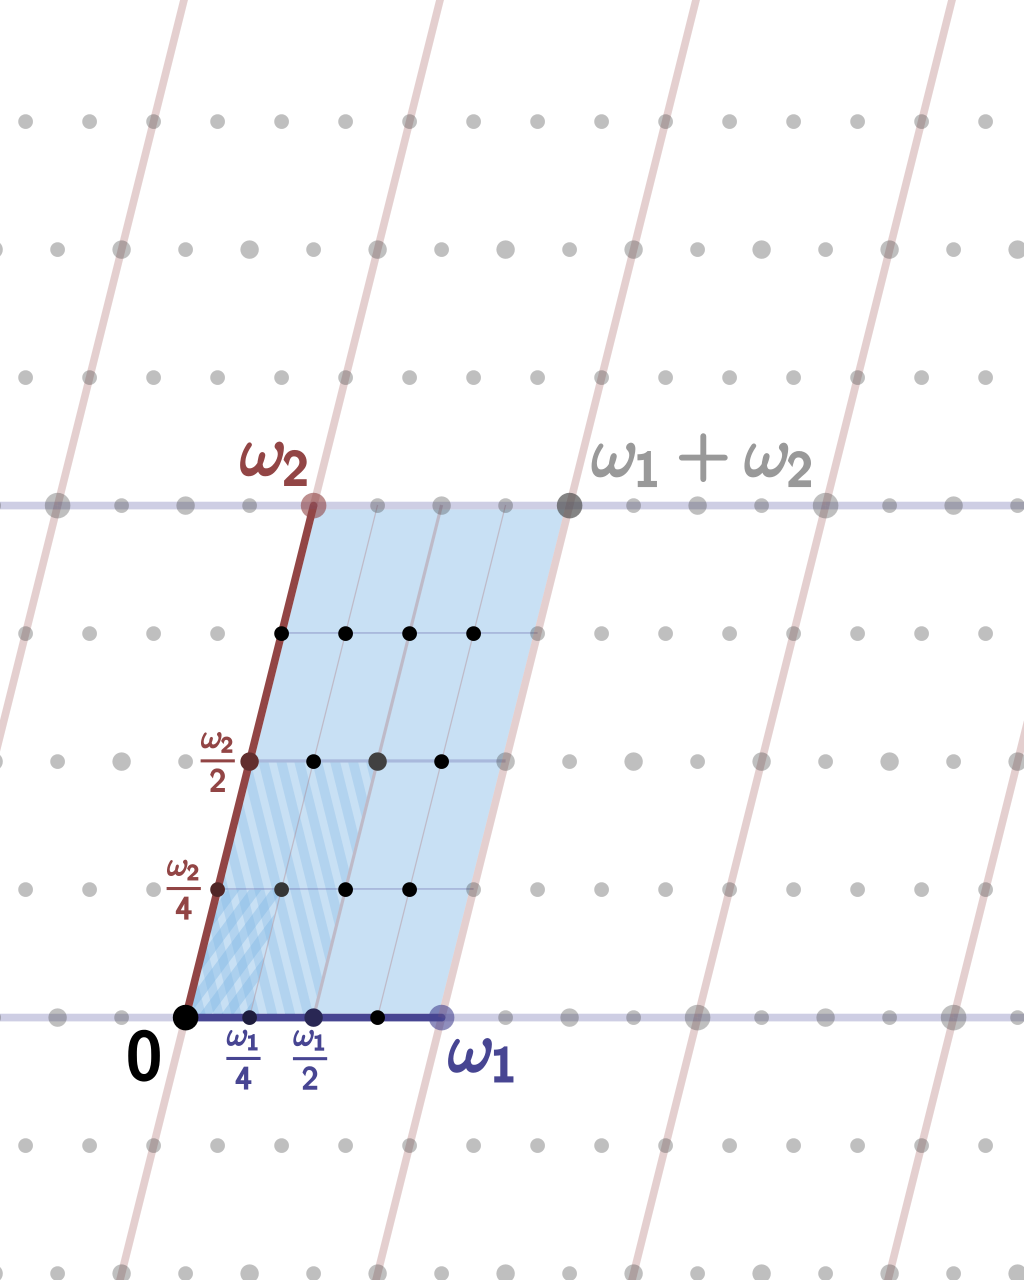
\includegraphics[width=0.25\textheight]{images/lattice.png} \qquad\qquad
	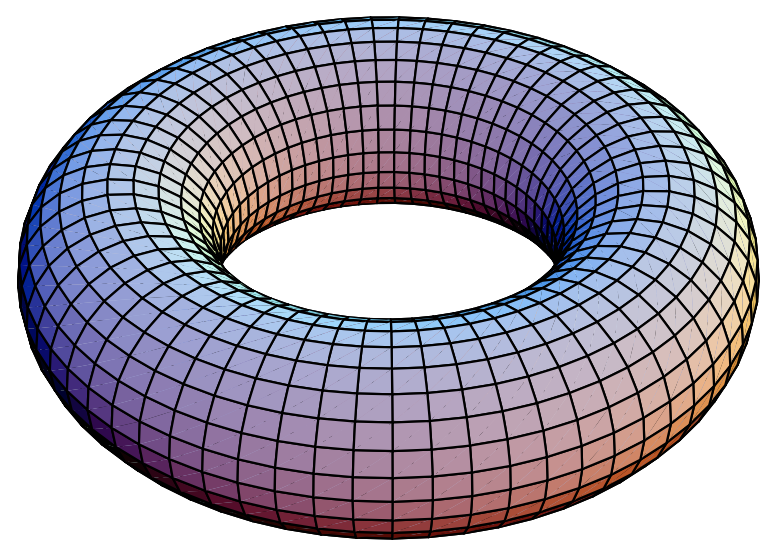
\includegraphics[width=0.25\textwidth]{images/torus.png}
	\end{figure}\fn{\tiny S. Derbyshire, \emph{Lattice torsion points}. CC BY-SA 3.0}

	\begin{figure}[!ht]
	\centering
	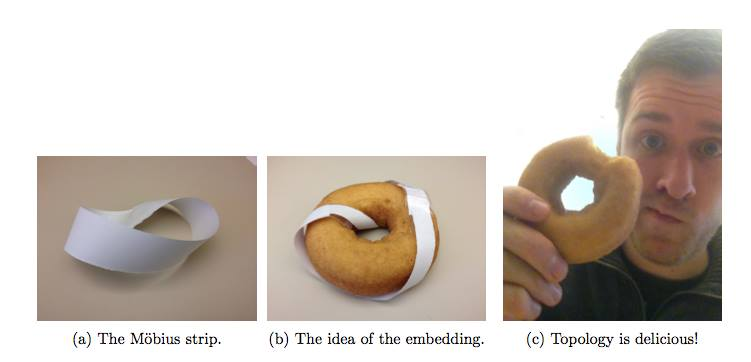
\includegraphics[width=0.8\textheight]{images/delicious.jpg}
	\end{figure}
\end{frame}



% Group Law
\begin{frame}[plain]
\ctext{The Group Law}
\end{frame}



% Groups
\begin{frame}[plain] \frametitle{What is a Group?} \small
\begin{dfn}[Group]
A group, $G$, is a set with a binary operation, $\star$, such that\dots
	\begin{enumerate}[(a)]
	\item (Associativity) $g \star (h \star k)= (g \star h) \star k$ for all $g, h, k \in G$.
	\item (Identity) There exists $e \in G$ such that $e \star g= g \star e= g$ for all $g \in G$.
	\item (Inverses) For every $g \in G$, there exists $g^{-1} \in G$ such that $g \star g^{-1}= g^{-1} \star g= e$. 
	\end{enumerate}
\end{dfn}

\begin{ex}
\begin{enumerate}[(i)]
\item The integers under addition modulo $n$ form a group, i.e. `clock arithmetic.' 
	\[
	\begin{tikzpicture}[scale=0.7]
        \draw[thick,SwarthGarnet] (0,0) circle (1);
        \draw[thick,SwarthGarnet] (0.8,0) -- (1,0);
        \draw[thick,SwarthGarnet] (0.693,0.4) -- (0.867,0.5);
        \draw[thick,SwarthGarnet] (0.4,0.693) -- (0.5,0.866);
        \draw[thick,SwarthGarnet] (0,0.8) -- (0,1);
        \draw[thick,SwarthGarnet] (-0.4,0.692) -- (-0.5,0.866);
        \draw[thick,SwarthGarnet] (-0.693,0.4) -- (-0.866,0.5);
        \draw[thick,SwarthGarnet] (-0.8,0) -- (-1,0); 
        \draw[thick,SwarthGarnet] (-0.693,-0.4) -- (-0.866,-0.5);
        \draw[thick,SwarthGarnet] (-0.4,-0.693) -- (-0.5,-0.866);
        \draw[thick,SwarthGarnet] (0,-0.8) -- (0,-1);
        \draw[thick,SwarthGarnet] (0.4,-0.693) -- (0.5,-0.866);
        \draw[thick,SwarthGarnet] (0.692,-0.4) -- (0.866,-0.5);
        
        \draw[fill=blue] (0,0) circle (0.05);
        
        \draw[very thick,white] (0,0) -- (0.247,0.761);
        \draw[thick,blue] (0,0) -- (0.247,0.761);
        
        \draw[very thick,white] (0,0) -- (0.298,-0.183);
        \draw[thick,blue] (0,0) -- (0.298,-0.183);
        \end{tikzpicture}
        \]

\item The integers, $\mathbb{Z}$, under addition form a group, i.e. an `infinite clock.'
\end{enumerate}
\end{ex}
\end{frame}



% Fields
\begin{frame}[plain] \frametitle{What is a (Galois) Field?} \footnotesize
\begin{dfn}[`Field']
A field is a collection of `numbers' where one can perform addition, subtraction, multiplication, and (nonzero) division and these operations are `nice.'
\end{dfn}

\begin{ex}
\begin{enumerate}[(i)]
\item The rational numbers, $\mathbb{Q}$, are a field with the usual $+, -, \times, \div$.
\item Number fields (extensions of $\mathbb{Q}$) are also fields. For example, consider $\Q(\sqrt{2})= \{ a + b \sqrt{2} \;|\; a, b \in \mathbb{Q} \}$,
	\[
	\begin{gathered}
	(5 - 3\sqrt{2}) + (-4 + 6 \sqrt{2})= 1 + 3 \sqrt{2} \\
	(6 - 7\sqrt{2}) \cdot (6 + 7\sqrt{2})= -62 + 0\sqrt{2} \\
	\dfrac{1 + 3\sqrt{2}}{1 + \sqrt{2}}= 5 - 2\sqrt{2}
	\end{gathered}
	\] 
The dimension of a number field as a $\mathbb{Q}$-vector space, i.e. number of `pieces' in these numbers, is called the \textit{degree} of the extension. 
\end{enumerate}
\end{ex}
\end{frame}



% Galois Fields
\begin{frame}[plain] \frametitle{Galois Fields} \footnotesize
\begin{dfn}[Galois Field]
A Galois field is a `number field' whose numbers satisfy extra symmetries. 
\end{dfn}

\begin{ex}
Consider the number field $\mathbb{Q}(i) = \{ a + bi \;|\; a, b \in \mathbb{Q} \}$, i.e. ``complex numbers with only rational parts.'' We can add, subtract, multiply, and divide these numbers. But they also have an extra symmetry given by conjugation, $\overline{a + bi}= a - bi$.
	\[
	\fbox{
	\begin{tikzpicture}[scale=0.72,every node/.style={scale=0.5}]
	\begin{axis}[
	grid=both,
	axis lines=middle,
	ticklabel style={fill=Topazolite!5!white},
	xmin= -10.5, xmax=10.5,
	ymin= -10.5, ymax=10.5,
	xtick={-10,-8,-6,-4,-2,0,2,4,6,8,10},
	ytick={-10,-8,-6,-4,-2,0,2,4,6,8,10},
	minor tick = {-10,-9,...,10},
	xlabel=\(x\),ylabel=\(y\),
	]
	\draw[draw=none,fill=red] (4,5) circle (0.25);
	\draw[dotted,red,thick] (0,0) -- (4,5);
	\node at (5.6,5.8) {\LARGE $4 + 5i$};

	\draw[draw=none,fill=blue] (4,-5) circle (0.25);
	\draw[dotted,blue,thick] (0,0) -- (4,-5);
	\node at (5.6,-6.2) {\LARGE $4 - 5i$};
	\end{axis}
	\end{tikzpicture}
	}
	\] 
\end{ex}
\end{frame}



% Addition Law
\begin{frame}
	\begin{figure}[h]
	\centering
	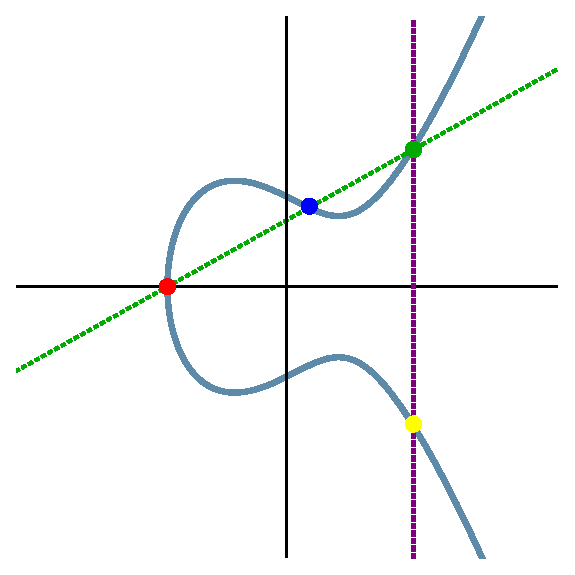
\includegraphics[width=0.75\textwidth]{images/ec_add.eps}
	\end{figure}
\end{frame}



% Why EC
\begin{frame}[plain]
\ctext{Why Elliptic Curves?}
\end{frame}



% Congruent Number Problem
\begin{frame} \frametitle{Congruent Number Problem} \scriptsize
An integer is a \textit{congruent number} if it is the area of a rational right triangle. \par\vspace{0.5\baselineskip}

\begin{minipage}{0.5\textwidth}
This is equivalent to finding a rational triplet $(x,y,z)$ with\dots
	\[
	x^2 + y^2= z^2 \quad \text{ and } \quad n= \dfrac{xy}{2}.
	\] 
\end{minipage}\begin{minipage}{0.5\textwidth}
\end{minipage}\begin{minipage}{0.5\textwidth}
	\[
	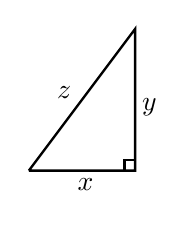
\begin{tikzpicture}[scale=0.9]
	\draw[line width=0.03cm] (0,0) -- (1.5,0) -- (1.5,2) -- (0,0);
	\draw[line width=0.03cm] (1.35,0) -- (1.35,0.15) -- (1.5,0.15);
	\node at (0.8,-0.2) {$x$};
	\node at (1.7,0.9) {$y$};
	\node at (0.5,1.1) {$z$};
	\end{tikzpicture}
	\]
\end{minipage}

\begin{ex}
\begin{itemize} \scriptsize
\item 6 is congruent: $3^2 + 4^2= 5^2$ and $\frac{3 \cdot 4}{2} = 6$
\item 5 is congruent: $\left( \frac{3}{2} \right)^2 + \left( \frac{20}{3} \right)^2= \left( \frac{41}{6} \right)^2$ and $\frac{1}{2} \left( \frac{3}{2} \cdot \frac{20}{3} \right)= 5$
\item 1 is \emph{not} congruent (due to Fermat) 
\item 157 is congruent (due to Don Zagier): \par\vspace{0.1cm}
		\scalebox{0.63}{$
	x= \dfrac{411340519227716149383203}{21666555693714761309610}, 
	y= \dfrac{6803298487826435051217540}{411340519227716149383203}, 
	z= \dfrac{224403517704336969924557513090674863160948472041}{8912332268928859588025535178967163570016480830}$
	}
\end{itemize}
\end{ex}

This problem is `equivalent' to finding rational points $(x, y)$ on the elliptic curve\dots
	\[
	y^2 = x^3 - n^2x
	\]

\end{frame}



% Fermat's Last Theorem
\begin{frame} \frametitle{Fermat's Last Theorem}
\small 

% Fermat Photos & Quotes
\begin{minipage}{0.33\textwidth}
\tiny
\begin{quote}
Cubum autem in duos cubos, aut quadratoquadratum in duos quadratoquadratos \& generaliter nullam in infinitum ultra quadratum potestatem in duos eiusdem nominis fas est dividere cuius rei demonstrationem mirabilem sane detexi. Hanc marginis exiguitas non caperet. \vspace{0.33cm}
\end{quote} 
\end{minipage}\begin{minipage}{0.33\textwidth}
	\begin{figure}
	\captionsetup{labelformat=empty}
	\centering
	\fbox{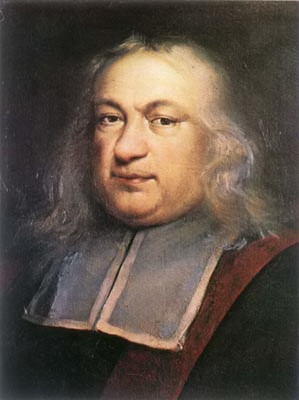
\includegraphics[width=0.55\textwidth]{images/fermat.jpeg}}
	\caption{\hspace{0.1cm}\tiny Pierre de Fermat}
	\end{figure}
\end{minipage}\begin{minipage}{0.33\textwidth} \tiny
\begin{quote}
``It is impossible to separate a cube into two cubes, or a fourth power into two fourth powers, or in general, any power higher than the second, into two powers. I have discovered a truly marvelous proof of this, which this margin is too narrow to contain.'' \vspace{0.9cm}
\end{quote}
\end{minipage}

% Theorem
\begin{thm}[{\small Fermat's Last Theorem; Wiles, 1994; Taylor-Wiles, 1995}]
There are no nontrivial integer solutions to the equation $x^n + y^n= z^n$ whenever $n > 2$.
\end{thm}

% Wiles - Taylor Photo
	\begin{figure}[h]
	\centering
	\begin{subfigure}{0.3\textwidth}
	\captionsetup{labelformat=empty}
	\centering
	\fbox{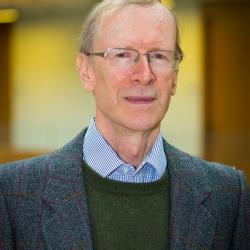
\includegraphics[width=0.64\textwidth]{images/wiles.jpg}}
	\caption{\scriptsize Andrew Wiles}
	\end{subfigure}
	%
	\begin{subfigure}{0.3\textwidth}
	\captionsetup{labelformat=empty}
	\centering
	\fbox{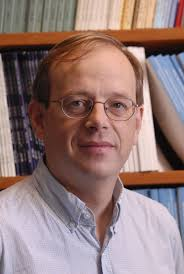
\includegraphics[width=0.43\textwidth]{images/taylor.jpeg}}
	\caption{\scriptsize Richard Taylor}
	\end{subfigure}
	\end{figure}

\end{frame}



% Sum of Three Cubes
\begin{frame}[plain,t] \frametitle{What integers are the sums of cubes?} \footnotesize
What integers $n$ are the sum of three cubes?
	\[
	x^3 + y^3 + z^3= n
	\]
\end{frame}



% Sum of Three Cubes
\begin{frame}[plain,t] \frametitle{What integers are the sums of cubes?} \footnotesize
What integers $n$ are the sum of three cubes?
	\[
	x^3 + y^3 + z^3= \xout{n} \; N
	\]
\end{frame}



% Sum of Three Cubes
\begin{frame} \frametitle{What integers are the sums of cubes?} \footnotesize
	\[
	x^3 + y^3 + z^3= N
	\] \pspace

{\color{SwarthGarnet} \textbullet} From 1955 -- 2016, it was known that all integers 1--100 that were not 4 or 5 modulo 9 were the sum of three cubes except 33, 42, 74. \pspace

{\color{SwarthGarnet} \textbullet} After the release of a Numberphile video, Huisman 2016 found the following:
	{\footnotesize
	\[
	(66\,229\,832\,190\,556)^3 + (28\,3450\,105\,697\,727)^3 + (-284\,650\,292\,555\,885)^3= 74
	\]
	} \pspace
	
{\color{SwarthGarnet} \textbullet} In 2019, Booker found the following:
	{\footnotesize
	\[
	(-2\,736\,111\,468\,807\,040)^3 + (-8\,778\,405\,442\,862\,239)^3 + (8\,866\,128\,975\,287\,528)^3= 33
	\]
	} \pspace
	
{\color{SwarthGarnet} \textbullet} Finally, shortly thereafter in 2019, Sutherland and Booker (using 1.3~million hours of computing time)
	{\footnotesize
	\[
	(12\,602\,123\,297\,335\,631)^3 + (80\,435\,758\,145\,817\,515)^3 + (-80\,538\,738\,812\,075\,974)^3= 42
	\]
	}
\end{frame}



% ECDH, Playstation, Bitcoin
\begin{frame}[plain] \frametitle{ECDH, Playstation 3, \& Bitcoin} \footnotesize
Elliptic curves are the basis for ECDH (Elliptic-Curve Diffie-Hellman) encryption, which is the backbone of most modern encryption (for now\dots). 
	\begin{figure}[h]
	\centering
	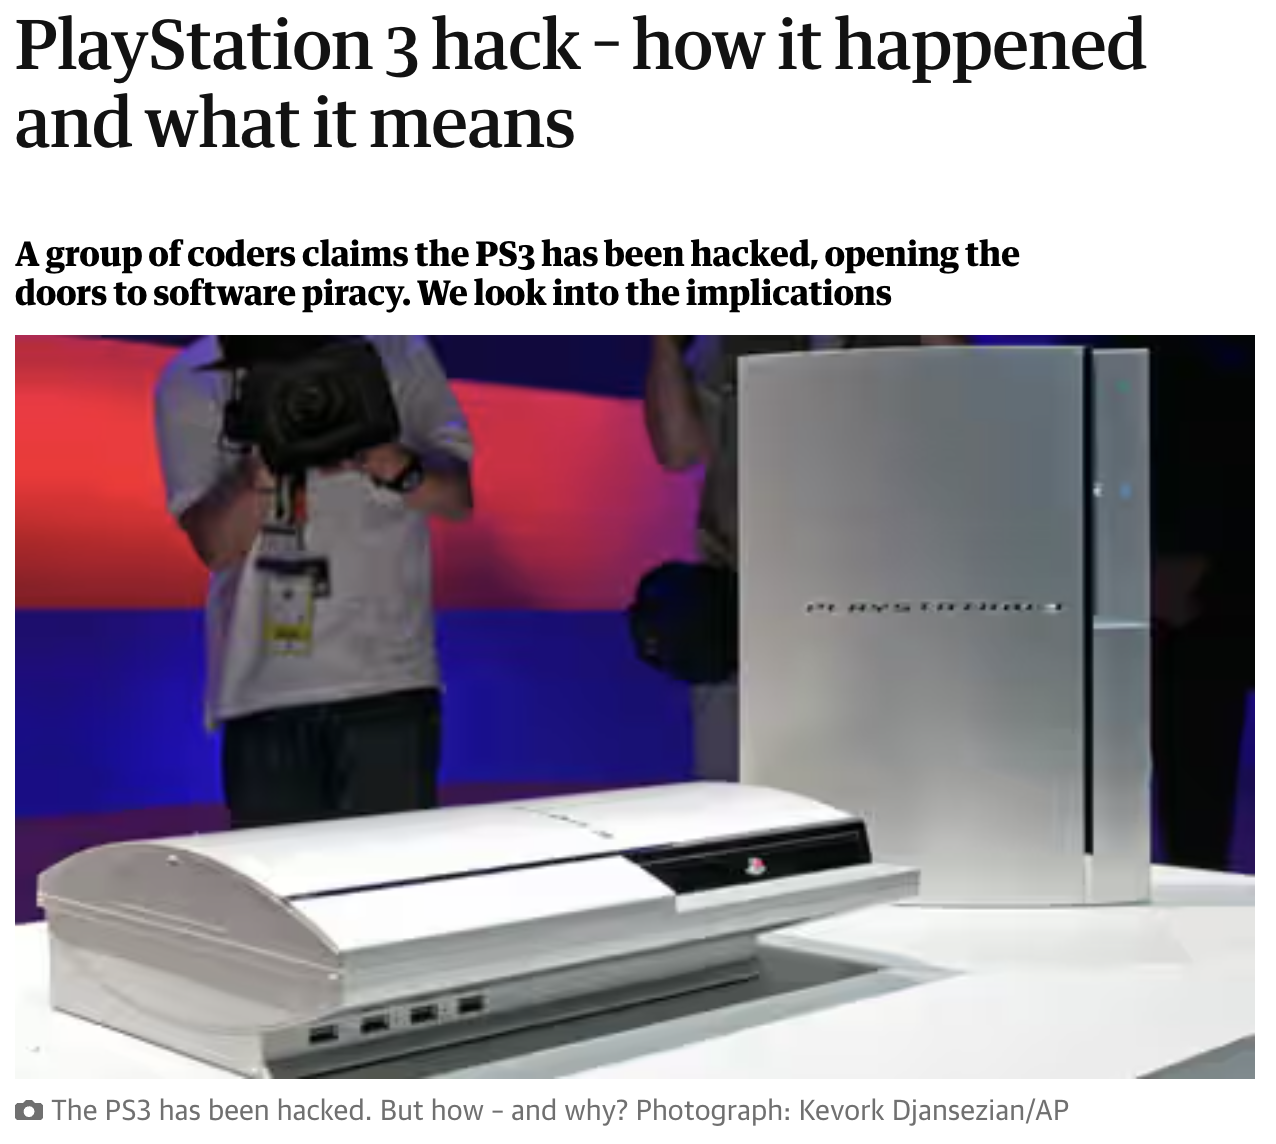
\includegraphics[width=0.515\textwidth]{images/playstation.png}
	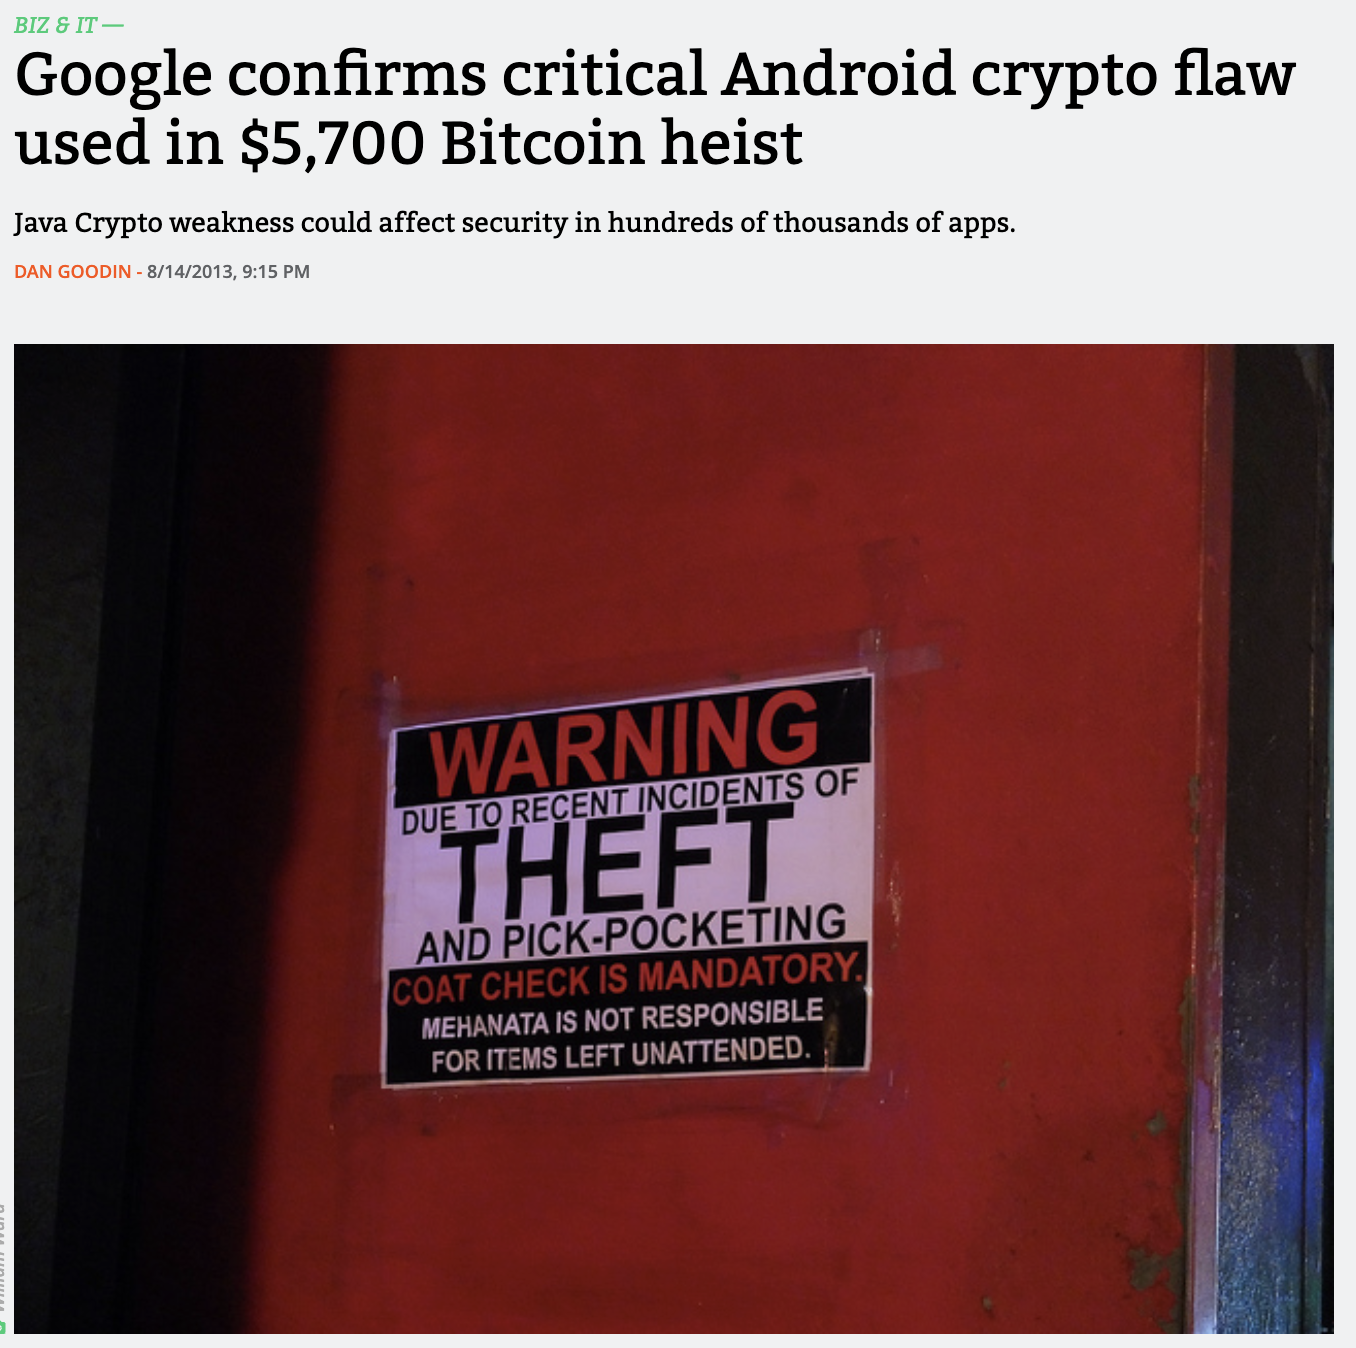
\includegraphics[width=0.475\textwidth]{images/bitcoin.png}
	\end{figure}
\end{frame}



% String Theory
\begin{frame}[plain] \frametitle{String Theory} \footnotesize
In String Theory, the idea of point-like particles are replaced by curve-like strings of some higher dimension, e.g. 6-dimensional or 23-dimensional. A single string which `moves about' and eventually returns to its start traces out a surface---specifically a torus! So paths of single strings `look like' elliptic curves! 
	\begin{figure}[ht]
	\centering
	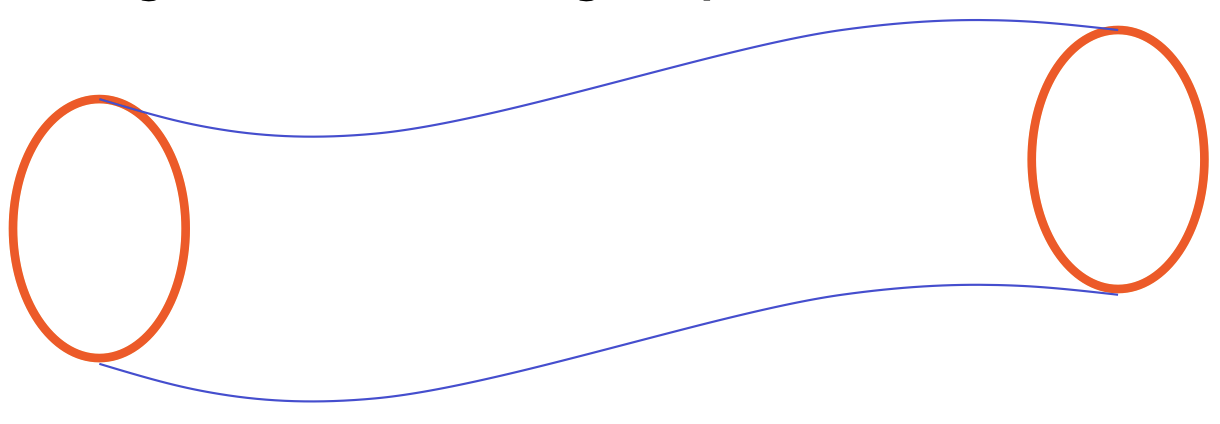
\includegraphics[width=0.35\textwidth]{images/stringpath.png}
	\end{figure}
Furthermore, in Quantum Physics, physicists often need to compute averages over all possible paths. So when considering this type of computation in String Theory, one would then be integrating over the space of all elliptic curves!
	\begin{figure}[ht]
	\centering
	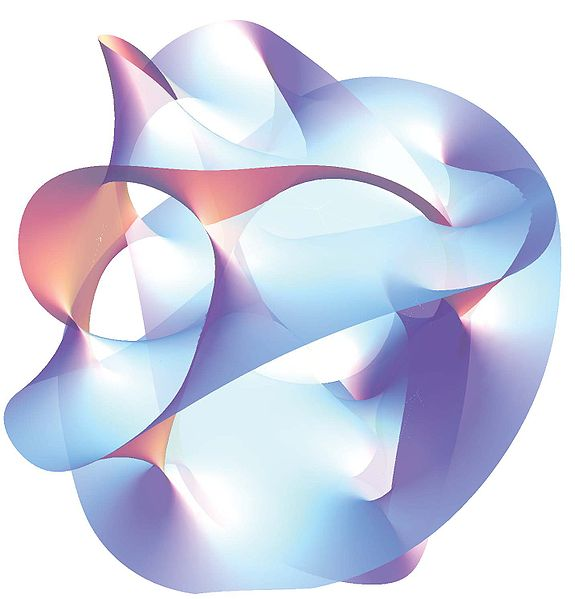
\includegraphics[width=0.30\textwidth]{images/calabi-yau.jpeg}
	\end{figure}
\end{frame}



% Moonshine
\begin{frame}[plain] \frametitle{Monstrous Moonshine} \scriptsize
An elliptic curve can be uniquely identified (over $\mathbb{C}$) by its $j$-invariant. The $j$-invariant is given by the modular $j$-invariant function,
	\[
	j(\tau)= \dfrac{1}{q} + 744 + 196884q + 214937609q^2 + \cdots
	\]
where $q= e^{2\pi i \tau}$ and $\tau$ is given by the elliptic curve. \pspace

	\begin{figure}[h]
	\centering
	\begin{subfigure}{0.20\textwidth}
	\captionsetup{labelformat=empty}
	\centering
	\fbox{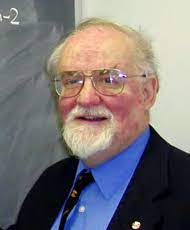
\includegraphics[width=0.62\textwidth]{images/mckay.jpeg}}
	\caption{\tiny John McKay}
	\end{subfigure} \quad
	%
	\begin{subfigure}{0.20\textwidth}
	\captionsetup{labelformat=empty}
	\centering
	\fbox{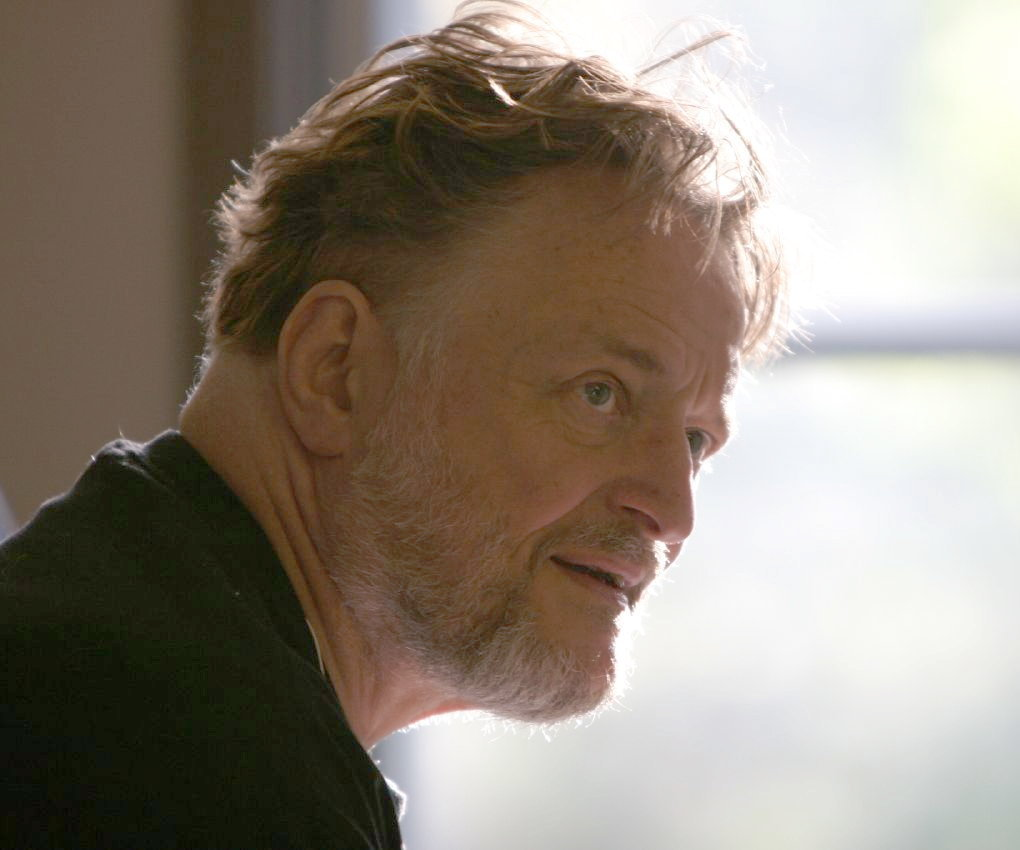
\includegraphics[width=0.9\textwidth]{images/conway.jpeg}}
	\caption{\tiny \hspace{0.2cm}John Conway}
	\end{subfigure}
	%
	\begin{subfigure}{0.20\textwidth}
	\captionsetup{labelformat=empty}
	\centering
	\fbox{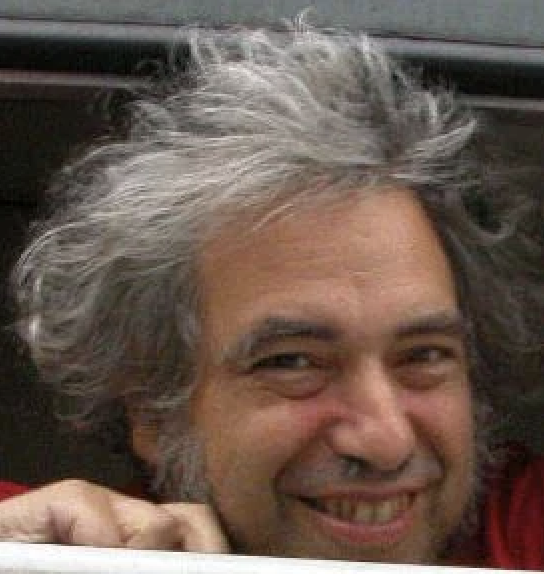
\includegraphics[width=0.71\textwidth]{images/norton.png}}
	\caption{\tiny \hspace{0.2cm}Simon Norton}
	\end{subfigure} \quad
	%
	\begin{subfigure}{0.20\textwidth}
	\captionsetup{labelformat=empty}
	\centering
	\fbox{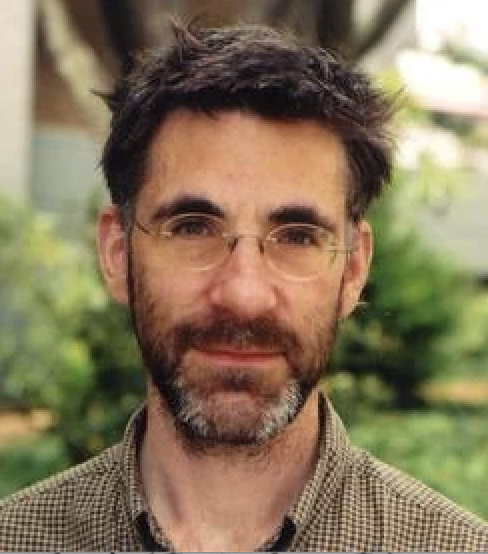
\includegraphics[width=0.665\textwidth]{images/borcherds.png}}
	\caption{\tiny Richard Borcherd65}
	\end{subfigure}
	\end{figure}

Beginning In 1978, John McKay, Conway-Norton, and Borcherds discovered that the coefficients in the modular $j$-invariant are sums of linear combinations of the dimensions of the irreducible representations of the monster group, $M$, which is the largest of the sporadic groups. These appear in the classification of all finite simple groups. In fact, Borcherd's work won a Field's Medal. \pspace

This is also related to the fact that\dots
	\[
	e^{\pi \sqrt{163}} \approx 262537412640768743.99999999999925007\dots
	\]
\end{frame}



% Art
\begin{frame}[plain] \frametitle{Art} \footnotesize
Lenstra \& de Smit were recently able to finish an incomplete piece of M.C. Escher using elliptic curves:
	\begin{figure}[ht]
	\centering
	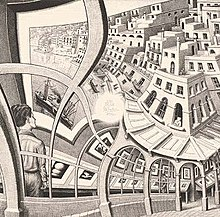
\includegraphics[width=0.482\textwidth]{images/escher2.jpg}
	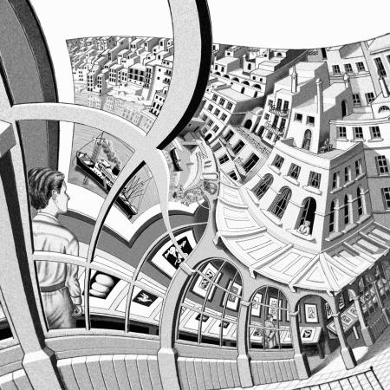
\includegraphics[width=0.478\textwidth]{images/escher_lenstra.jpeg}
	\end{figure}
\end{frame}



% Varying Problems
\begin{frame}[plain] \frametitle{The Numerous Problem Variations} \footnotesize
There are numerous questions you can ask about elliptic curves, e.g.
\begin{itemize}
\item Fix an elliptic curve, vary the extensions.
	\[
	\begin{tikzcd}[ampersand replacement=\&]
	E(K_1) \& E(K_2) \& \cdots \& E(K_n) \& \cdots \\
	\& \& E(F) \arrow[dash]{ull} \arrow[dash]{ul} \arrow[dash]{u} \arrow[dash]{ur} \arrow[dash]{urr} \& \& 
	\end{tikzcd}
	\]

\item Fix a field, $K$, and vary the elliptic curves:
	\[
	E_1(K) \qquad E_2(K) \qquad E_3(K) \qquad E_4(K) \qquad E_5(K) \qquad \cdots 
	\]

\item Vary both the curves and the fields:
	\begin{table}[ht]
	\centering
	\begin{tabular}{cccc}
	$E_1(K_1)$ & $E_1(K_2)$ & $E_1(K_3)$ & $\cdots$ \\
	$E_2(K_1)$ & $E_2(K_2)$ & $E_2(K_3)$ & $\cdots$ \\
	$E_3(K_1)$ & $E_3(K_2)$ & $E_3(K_3)$ & $\cdots$ \\
	$\vdots$ & $\vdots$ & $\vdots$ & $\ddots$
	\end{tabular}
	\end{table}
\end{itemize}
\end{frame}



% Lang Quote
{\setbeamertemplate{background canvas}{
\tikz[remember picture,overlay]
	\node[opacity=0.3] at (current page.center) {
	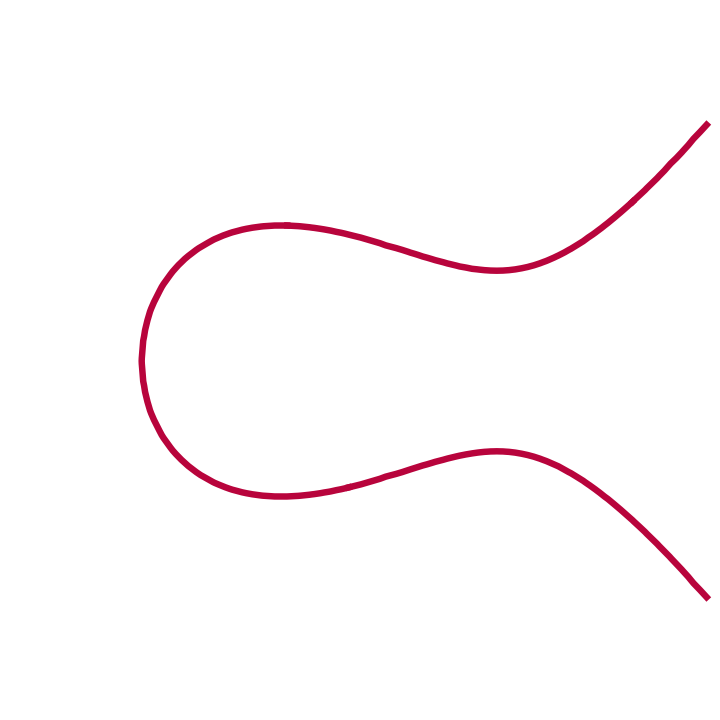
\includegraphics[width=1.25\paperwidth,
	height=1.25\paperheight]{images/curve2red.png}};} 
\begin{frame}[plain]
	\begin{minipage}{0.18\textwidth}
 	\begin{figure}[h]
	\centering
	\fbox{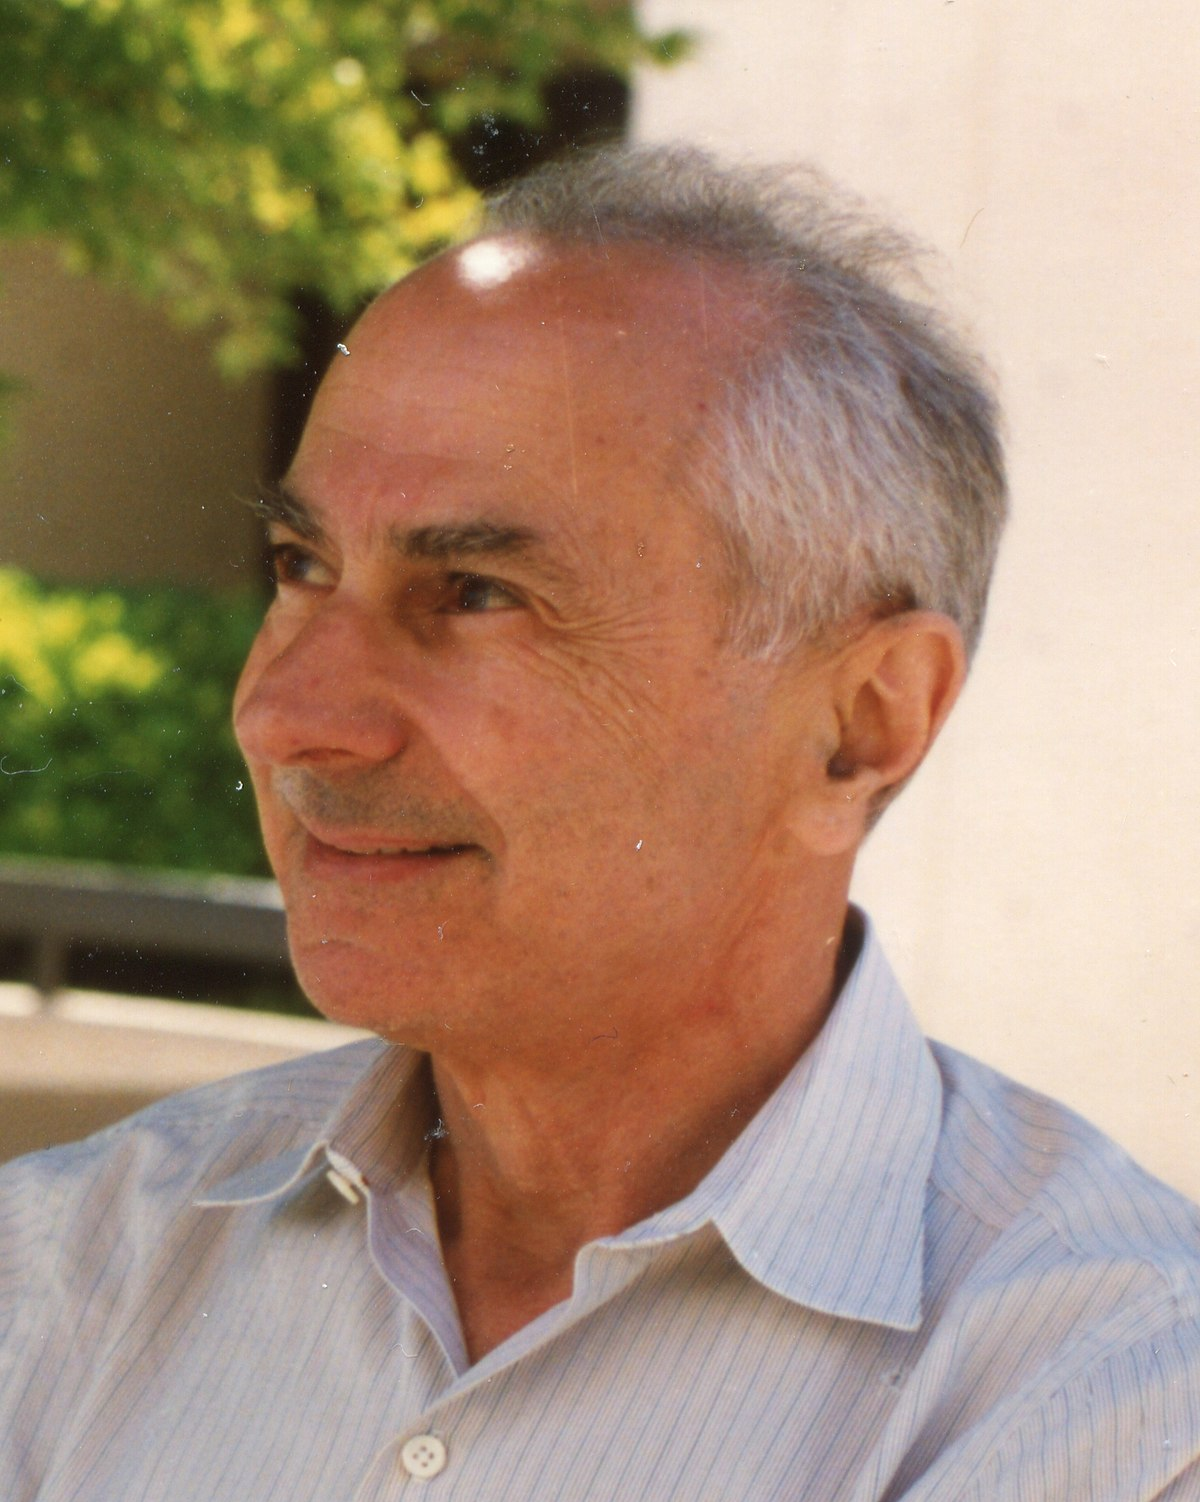
\includegraphics[width=1.1\textwidth]{images/lang.jpeg}} \par
	{\small 1927 -- 2005}
	\end{figure}
	\end{minipage} \hspace{0.2cm} \begin{minipage}{0.76\textwidth}
	\begin{center} \phantom{.} \par \phantom{.} \par
	{\itshape ``It is possible to write endlessly on elliptic curves. (This is not a threat.)''} \\
	 \phantom{x}\hfill-- Serge Lang, \textit{Elliptic Curves: Diophantine Analysis}
	\end{center}
 	\end{minipage}
\end{frame}
}



% What about Structure?
\begin{frame}[plain]
\ctext{Elliptic Curve Structure}
\end{frame}



% Mordell - Weil - Neron
\begin{frame}
	\begin{thm}[Mordell-Weil-N\'eron, 1952]
	Let $K$ be a field that is finitely generated over its prime field, and let $A/K$ be an abelian variety. Then the group of $K$-rational points on $A$, denoted $A(K)$, is a finitely generated abelian group. In particular,
		\[
		A(K) \cong \Z^{r_K} \oplus A(K)_\tors,
		\]
	where $r_K \geq 0$ is the rank and $A(K)_\tors$ is the torsion subgroup. 
	\end{thm}
	\begin{figure}[h]
	\centering
	\begin{subfigure}{0.3\textwidth}
	\captionsetup{labelformat=empty}
	\centering
	\fbox{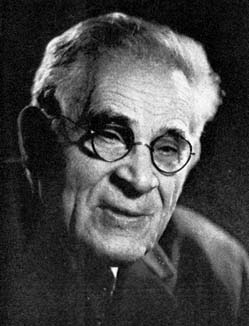
\includegraphics[width=0.8\textwidth]{images/mordell.jpg}}
	\caption{Louis J. Mordell}
	\end{subfigure}
	%
	\begin{subfigure}{0.3\textwidth}
	\captionsetup{labelformat=empty}
	\centering
	\fbox{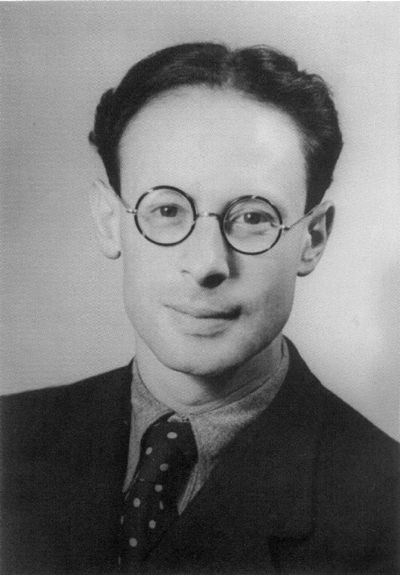
\includegraphics[width=0.74\textwidth]{images/weil.jpg}}
	\caption{Andr\'e Weil}
	\end{subfigure}
	%
	\begin{subfigure}{0.3\textwidth}
	\captionsetup{labelformat=empty}
	\centering
	\fbox{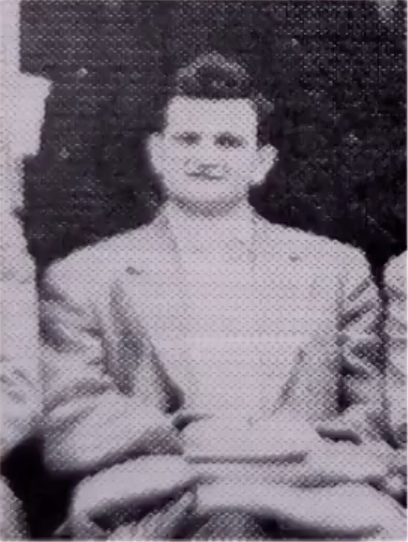
\includegraphics[width=0.8\textwidth]{images/neron.png}}
	\caption{Andr\'e N\'eron}
	\end{subfigure}
	\end{figure}
\end{frame}



% Ranks
\begin{frame}[plain] \frametitle{Ranks of Elliptic Curves (over $\Q$)}

\begin{minipage}{0.45\textwidth}
	\begin{table}[h]
	\centering
	\resizebox{!}{0.60\textwidth}{%
	\begin{tabular}{lll}  
	{\itshape\large\bfseries Rank} & {\itshape\large\bfseries Year} & {\itshape\large\bfseries Due To} \\ \hline
	3 & 1938 & Billing \\ \rowcolor{SwarthGarnet}
	\textcolor{Topazolite}{4} & \textcolor{Topazolite}{1945} &  \textcolor{Topazolite}{Wiman} \\ 
	6 & 1974 & Penney/Pomerance \\ \rowcolor{SwarthGarnet}
	\textcolor{Topazolite}{7} & \textcolor{Topazolite}{1975} & \textcolor{Topazolite}{Penney/Pomerance} \\
	8 & 1977 & Grunewald/Zimmert \\ \rowcolor{SwarthGarnet}
	\textcolor{Topazolite}{9} & \textcolor{Topazolite}{1977} & \textcolor{Topazolite}{Brumer/Kramer} \\
	12 & 1982 & Mestre \\ \rowcolor{SwarthGarnet}
	\textcolor{Topazolite}{14} & \textcolor{Topazolite}{1986} & \textcolor{Topazolite}{Mestre} \\
	15 & 1992 &  Mestre \\  \rowcolor{SwarthGarnet}
	\textcolor{Topazolite}{17} & \textcolor{Topazolite}{1992} & \textcolor{Topazolite}{Nagao} \\
	19 & 1992 & Fermigier \\ \rowcolor{SwarthGarnet}
	\textcolor{Topazolite}{20} & \textcolor{Topazolite}{1993} & \textcolor{Topazolite}{Nagao} \\
	21 & 1994 & Nagao/Kouya \\ \rowcolor{SwarthGarnet}
	\textcolor{Topazolite}{22} & \textcolor{Topazolite}{1997} & \textcolor{Topazolite}{Fermigier} \\
	23 & 1998 & Martin/McMillen \\ \rowcolor{SwarthGarnet}
	\textcolor{Topazolite}{24} & \textcolor{Topazolite}{2000} & \textcolor{Topazolite}{Martin/McMillen} \\
	28 & 2006 & Elkies 
	\end{tabular}
	}
	\end{table}
\end{minipage} \qquad \begin{minipage}{0.45\textwidth}
	\begin{figure}
	\centering
	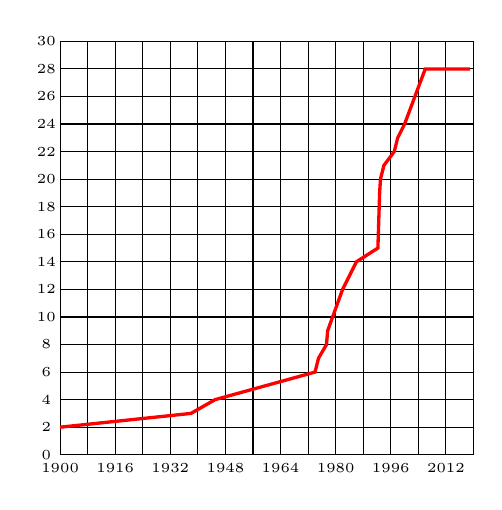
\begin{tikzpicture}[scale=0.35]%[scale=0.50, every node/.style={scale=0.1}]
	\foreach \k in {0,...,15}
		{
		\draw (\k,0) -- (\k,15);
		}
	\foreach \k in {0,...,15}
		{
		\draw (0,\k) -- (15,\k);
		}
	\node at (0,-0.5) {\tiny 1900};
	\node at (2,-0.5) {\tiny 1916};
	\node at (4,-0.5) {\tiny 1932};
	\node at (6,-0.5) {\tiny 1948};
	\node at (8,-0.5) {\tiny 1964};
	\node at (10,-0.5) {\tiny 1980};
	\node at (12,-0.5) {\tiny 1996};
	\node at (14,-0.5) {\tiny 2012};
	
	\node at (-0.5,0) {\tiny 0};
	\node at (-0.5,1) {\tiny 2};
	\node at (-0.5,2) {\tiny 4};
	\node at (-0.5,3) {\tiny 6};
	\node at (-0.5,4) {\tiny 8};
	\node at (-0.5,5) {\tiny 10};
	\node at (-0.5,6) {\tiny 12};
	\node at (-0.5,7) {\tiny 14};
	\node at (-0.5,8) {\tiny 16};
	\node at (-0.5,9) {\tiny 18};
	\node at (-0.5,10) {\tiny 20};
	\node at (-0.5,11) {\tiny 22};
	\node at (-0.5,12) {\tiny 24};
	\node at (-0.5,13) {\tiny 26};
	\node at (-0.5,14) {\tiny 28};
	\node at (-0.5,15) {\tiny 30};
	
	\draw[very thick,red] plot[samples=500] coordinates {
	(0,1)
	(4.75,1.5)
	(5.625,2)
	(9.25,3)
	(9.375,3.5)
	(9.6667,4)
	(9.7083,4.5)
	(10.25,6)
	(10.75,7)
	(11.5313,7.5)
	(11.5625,8.5)
	(11.5938,9.5)
	(11.625,10)
	(11.75,10.5)
	(12.125,11)
	(12.25,11.5)
	(12.5,12)
	(13.25,14)
	(14.875,14)
	};
	\end{tikzpicture}
	\end{figure}
\end{minipage}
\end{frame}



% Torsion Subgroup
\begin{frame}[plain,fragile]
\ctext{Torsion Subgroups of Elliptic Curves} \small
\begin{tikzcd}[scale=0.5]
	& \left\{\begin{matrix} \text{Torsion Subgroups} \\ \text{of Elliptic Curves} \end{matrix} \right\} \arrow[<->]{dl} \arrow[<->]{dr} & \\
	\left\{\begin{matrix} \text{Galois} \\ \text{Representations} \end{matrix} \right\} \arrow[<->]{rr} & & \left\{\begin{matrix} \text{Modular} \\ \text{Curves} \end{matrix} \right\}
	\end{tikzcd}
\vfill
\end{frame}



% Q-Torsion (Mazur)
\begin{frame}[plain]
\begin{thm}[Levi-Ogg Conjecture; Mazur, 1977]
If $E/\Q$ is a rational elliptic curve, then the possible torsion subgroups $E(\Q)_\tors$ are precisely:
	\[
	\begin{cases}
	\Z/n\Z, & \text{with } n=1,2,\ldots,10,12 \text{ or} \\
	\Z/2\Z \oplus \Z/2n\Z, & \text{with } n=1,\ldots,4
	\end{cases}
	\]
Furthermore, each possibility occurs infinitely often.
\end{thm}
	\begin{figure}[h]
	\centering
	\begin{subfigure}{0.3\textwidth}
	\captionsetup{labelformat=empty}
	\centering
	\fbox{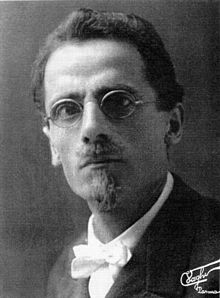
\includegraphics[width=0.72\textwidth]{images/levi.jpg}}
	\caption{Beppo Levi}
	\end{subfigure}
	%
	\begin{subfigure}{0.3\textwidth}
	\captionsetup{labelformat=empty}
	\centering
	\fbox{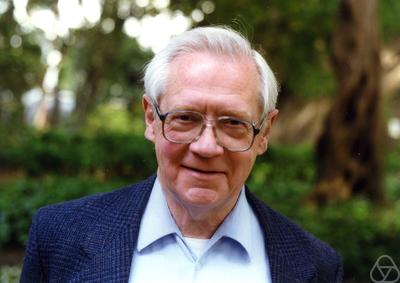
\includegraphics[width=\textwidth]{images/ogg.jpg}}
	\caption{Andrew Ogg}
	\end{subfigure} \hspace{0.05cm}
	%
	\begin{subfigure}{0.3\textwidth}
	\captionsetup{labelformat=empty}
	\centering
	\fbox{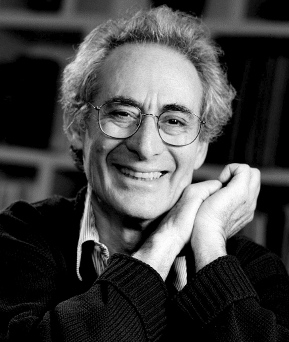
\includegraphics[width=0.83\textwidth]{images/mazur.jpg}}
	\caption{Barry Mazur}
	\end{subfigure}
	\end{figure}
\end{frame}



% Quadratic Rational EC
\begin{frame}[plain]
\footnotesize
\begin{thm}[Najman, 2015]
Let $E/\Q$ be a rational elliptic curve, and let $K/\Q$ be a quadratic number field. Then the possible torsion subgroups $E(K)_\tors$ are precisely:
	\[
	\begin{cases}
	\Z/n\Z, & \text{with } n= 1, 2, \ldots, 10, 12, 15, 16 \text{ or} \\
	\Z/2\Z \oplus \Z/2n\Z, & \text{with } n= 1, 2, \ldots, 6 \text{ or} \\
	\Z/3\Z \oplus \Z/3n\Z, & \text{with } n= 1, 2 \text{ or} \\
	\Z/4\Z \oplus \Z/4\Z
	\end{cases}
	\]
Each such possibility occurs for infinitely many elliptic curves except for $\Z/15\Z$, which occurs only for the elliptic curves \texttt{50b1} and \texttt{50a3} over $\Q(\sqrt{5})$ and the elliptic curves \texttt{50b2} and \texttt{450b4} over $\Q(\sqrt{-15})$. 
\end{thm}
	\begin{figure}[!ht]
	\centering
	\captionsetup{labelformat=empty}
	\fbox{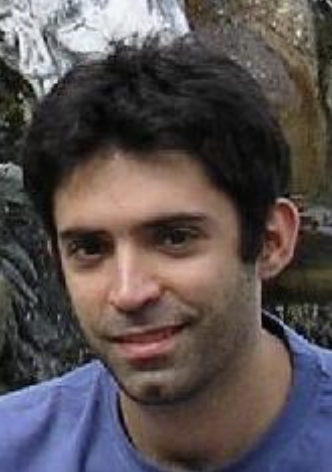
\includegraphics[width=0.18\textwidth]{images/najman2.png}}
	\caption{Filip Najman}
	\end{figure}
\end{frame}



% Cubic Rational EC
\begin{frame}[plain]
\begin{thm}[Najman, 2015]
Let $E/\Q$ be a rational elliptic curve, and let $K/\Q$ be a cubic number field. Then the possible torsion subgroups $E(K)_\tors$ are precisely:
	\[
	\begin{cases}
	\Z/n\Z, & \text{with } n= 1, 2, \ldots, 10, 12, 13, 14, 18, 21 \text{ or} \\
	\Z/2\Z \oplus \Z/2n\Z, & \text{with } n= 1, 2, 3, 4, 7
	\end{cases}
	\]
Each such possibility occurs for infinitely many elliptic curves except for $\Z/21\Z$, which only occurs for the elliptic curve \texttt{162b1} over $\Q(\zeta_9)^+$.
\end{thm}
	\begin{figure}[!ht]
	\centering
	\captionsetup{labelformat=empty}
	\fbox{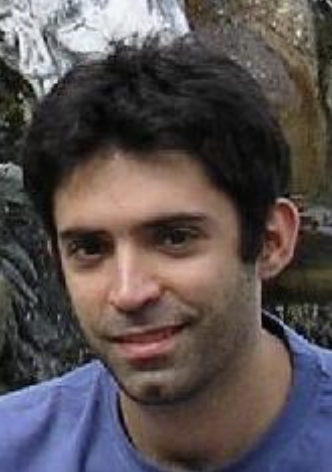
\includegraphics[width=0.18\textwidth]{images/najman2.png}}
	\caption{Filip Najman}
	\end{figure}
\end{frame}



% Quartic Rational EC
\begin{frame}[plain]
\footnotesize
\begin{thm}[Chou, 2015; Gonz\'alez-Jimenez, Lozano-Robledo, 2016; Gonz\'alez-Jimenez, Najman, 2016]
Let $E/\Q$ be a rational elliptic curve, and let $K/\Q$ be a quartic number field. Then the possible torsion subgroups $E(K)_\tors$ are precisely:
	\[
	\begin{cases}
	\Z/n\Z, & \text{with } n= 1, 2, \ldots, 10, 12, 13, 15, 16, 20, 24 \text{ or} \\
	\Z/2\Z \oplus \Z/2n\Z, & \text{with } n= 1, 2, \ldots, 6, 8 \text{ or} \\
	\Z/3\Z \oplus \Z/3n\Z, & \text{with } n= 1, 2 \text{ or} \\
	\Z/4\Z \oplus \Z/4n\Z, & \text{with } n= 1, 2 \text{ or} \\
	\Z/5\Z \oplus \Z/5\Z, & \text{or} \\
	\Z/6\Z \oplus \Z/6\Z 
	\end{cases}
	\]
Each such possibility occurs for infinitely many elliptic curves except for $\Z/15\Z$, which occurs only for the elliptic curves with $j(E) \in \{ -5^2/2, -5^2 \cdot 241^3/2^3$, $-5 \cdot 29^3/2^5, 5 \cdot 211^3/2^{15} \}$ over some quartic field. 
\end{thm}
	\begin{figure}[h]
	\centering
	\begin{subfigure}{0.20\textwidth}
	\captionsetup{labelformat=empty}
	\centering
	\fbox{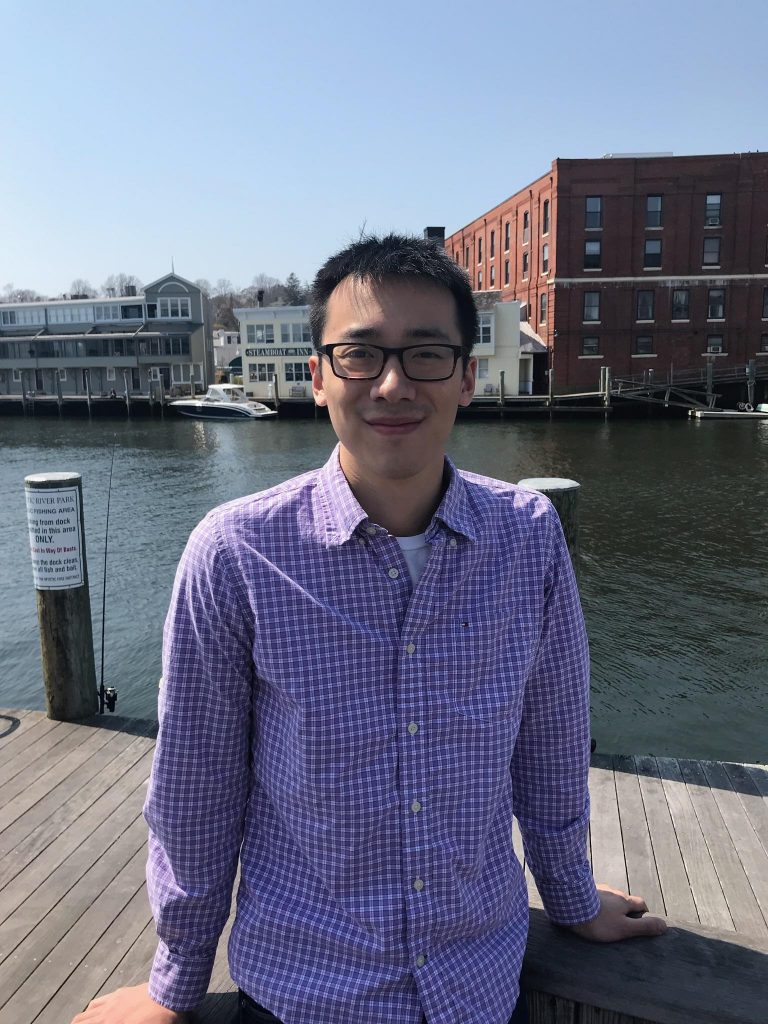
\includegraphics[width=0.62\textwidth]{images/chou.jpg}}
	\caption{\tiny Michael Chou}
	\end{subfigure} \quad
	%
	\begin{subfigure}{0.20\textwidth}
	\captionsetup{labelformat=empty}
	\centering
	\fbox{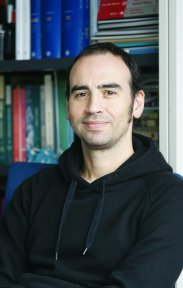
\includegraphics[width=0.45\textwidth]{images/jimenez2.jpeg}}
	\caption{\tiny \hspace{0.7cm}Enrique \\ \;\;\;Gonz\'alez-Jim\'enez}
	\end{subfigure}
	%
	\begin{subfigure}{0.20\textwidth}
	\captionsetup{labelformat=empty}
	\centering
	\fbox{
\includegraphics[width=0.72\textwidth]{images/robledo.jpg}}
	\caption{\tiny \hspace{0.7cm}\'Alvaro \\ \;\;\;\;\;Lozano-Robledo}
	\end{subfigure} \quad
	%
	\begin{subfigure}{0.20\textwidth}
	\captionsetup{labelformat=empty}
	\centering
	\fbox{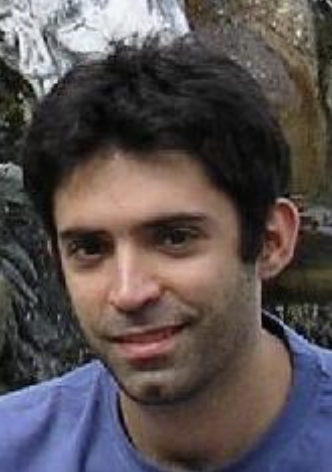
\includegraphics[width=0.58\textwidth]{images/najman2.png}}
	\caption{\tiny Filip Najman}
	\end{subfigure}
	\end{figure}
\end{frame}



% Quintic Rational EC
\begin{frame}[plain]
\begin{thm}[Gonz\'alez-Jimenez, 2016]
Let $E/\Q$ be a rational elliptic curve, and let $K/\Q$ be a quintic number field. Then the possible torsion subgroups $E(K)_\tors$ are precisely:
	\[
	\begin{cases}
	\Z/n\Z, & \text{with } n= 1, 2, \ldots, 12, 25 \text{ or} \\
	\Z/2\Z \oplus \Z/2n\Z, & \text{with } n= 1, 2, 3, 4
	\end{cases}
	\]
Each of these possibilities occurs infinitely many times except for $\Z/11\Z$ which occurs for the elliptic curves \texttt{121a2}, \texttt{121c2}, and \texttt{121b1} over some quintic field. 
\end{thm}
	\begin{figure}[!ht]
	\centering
	\captionsetup{labelformat=empty}
	\fbox{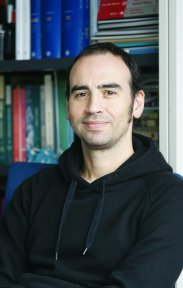
\includegraphics[width=0.18\textwidth]{images/jimenez2.jpeg}}
	\caption{Enrique Gonz\'alez-Jim\'enez}
	\end{figure}
\end{frame}



% Sextic Rational EC
\begin{frame}[plain]
\footnotesize
\begin{thm}[Daniels, Gonz\'alez-Jimenez, 2018; Gu{\u{z}}vi\'c, 2019]
Let $E/\Q$ be a rational elliptic curve, and let $K/\Q$ be a sextic number field. Then the possible torsion subgroups $E(K)_\tors$ are among:
	\[
	\begin{cases}
	\Z/n\Z, & \text{with } n= 1, 2, \ldots, 16, 18, 21, 30, n \neq 11  \text{ or} \\
	\Z/2\Z \oplus \Z/2n\Z, & \text{with } n= 1, 2, \ldots, 7, 9 \text{ or} \\
	\Z/3\Z \oplus \Z/3n\Z, & \text{with } n= 1, 2, 3, 4, 6^* \text{ or} \\
	\Z/4\Z \oplus \Z/4n\Z, & \text{with } n= 1, 3 \\
	\Z/6\Z \oplus \Z/6\Z 
	\end{cases}
	\]
Each such possibility occurs for infinitely many elliptic curves except for $\Z/15\Z$, $\Z/21\Z$, $\Z/30\Z$, $\Z/4\Z \oplus \Z/12\Z$, and possibly $\Z/3\Z \oplus \Z/18\Z$. 
\end{thm}
	\begin{figure}[h]
	\centering
	\begin{subfigure}{0.30\textwidth}
	\captionsetup{labelformat=empty}
	\centering
	\fbox{
\includegraphics[width=0.63\textwidth]{images/daniels.jpeg}}
	\caption{\tiny Harris Daniels}
	\end{subfigure} 
	%
	\begin{subfigure}{0.30\textwidth}
	\captionsetup{labelformat=empty}
	\centering
	\fbox{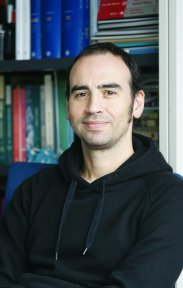
\includegraphics[width=0.40\textwidth]{images/jimenez2.jpeg}}
	\caption{\tiny Enrique Gonz\'alez-Jim\'enez}
	\end{subfigure}
	%
	\begin{subfigure}{0.30\textwidth}
	\captionsetup{labelformat=empty}
	\centering
	\fbox{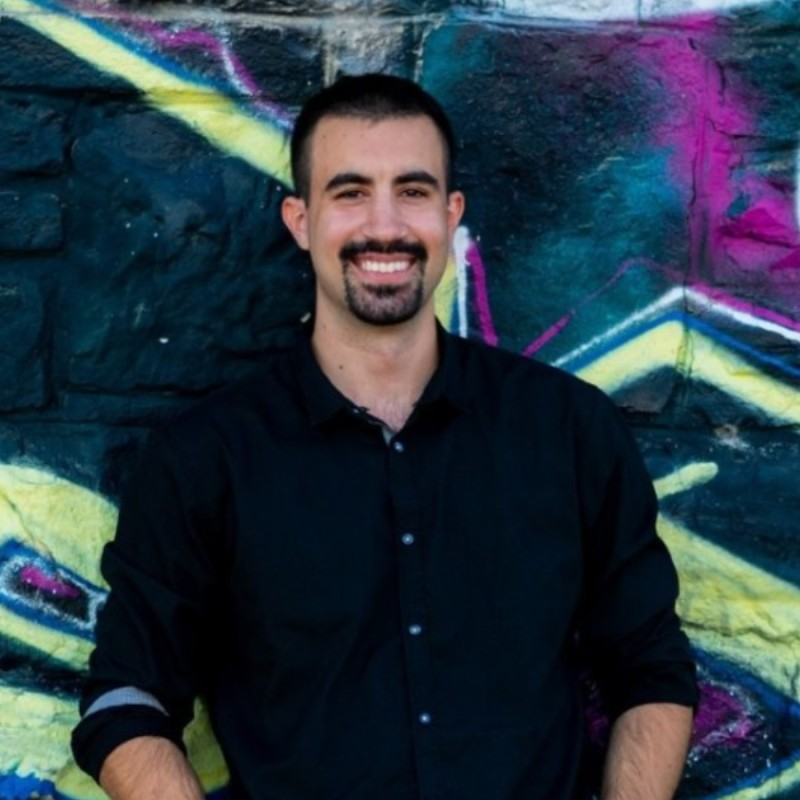
\includegraphics[width=0.635\textwidth]{images/tomislav.jpeg}}
	\caption{\tiny Tomislav Gu{\u{z}}vi\'c}
	\end{subfigure}
	\end{figure}
\end{frame}



% Other Fields Rational EC
\begin{frame}[plain]
\begin{thm}[Gonz\'alez-Jimenez, Najman, 2016]
Let $E/\Q$ be a rational elliptic curve, and let $K/\Q$ be a number field whose smallest prime divisor is at least 7, then the only possible torsion subgroups $E(\Q)_\tors$ are those from Mazur's list, namely:
	\[
	\begin{cases}
	\Z/n\Z, & \text{with } n= 1, 2, \ldots, 10, 12 \text{ or} \\
	\Z/2\Z \oplus \Z/2n\Z, & \text{with } n= 1, 2, 3, 4
	\end{cases}
	\]
Each such possibility occurs for infinitely many elliptic curves. In fact, if the largest prime divisor is at least 11, then $E(K)_\tors=$ $E(\Q)_\tors$. 
\end{thm}
	\begin{figure}[h]
	\centering
	\begin{subfigure}{0.40\textwidth}
	\captionsetup{labelformat=empty}
	\centering
	\fbox{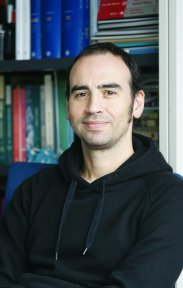
\includegraphics[width=0.40\textwidth]{images/jimenez2.jpeg}}
	\caption{\footnotesize \hspace{0.4cm} Enrique Gonz\'alez-Jim\'enez}
	\end{subfigure}
	%
	\begin{subfigure}{0.40\textwidth}
	\captionsetup{labelformat=empty}
	\centering
	\fbox{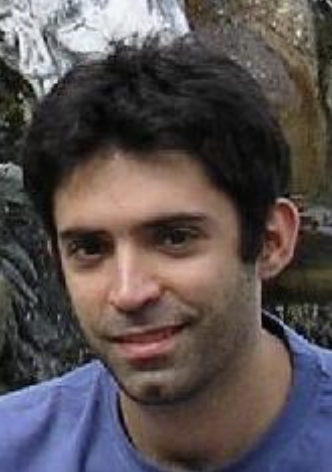
\includegraphics[width=0.45\textwidth]{images/najman2.png}}
	\caption{\footnotesize Filip Najman}
	\end{subfigure}
	\end{figure}
\end{frame}